\documentclass[output=paper,
modfonts
]{LSP/langsci}


%\usepackage{langsci-optional}
\usepackage{langsci-gb4e}
\usepackage{langsci-lgr}

\usepackage{listings}
\lstset{basicstyle=\ttfamily,tabsize=2,breaklines=true}

%added by author
% \usepackage{tipa}
\usepackage{multirow}
\graphicspath{{figures/}}
\usepackage{langsci-branding}

%
\newcommand{\sent}{\enumsentence}
\newcommand{\sents}{\eenumsentence}
\let\citeasnoun\citet

\renewcommand{\lsCoverTitleFont}[1]{\sffamily\addfontfeatures{Scale=MatchUppercase}\fontsize{44pt}{16mm}\selectfont #1}
  

\ChapterDOI{10.5281/zenodo.495451}
\title{Preliminaries to the investigation of clitic sequencing in Greek and Indo-Iranian}

\author{%
 Mark Hale\affiliation{Concordia University, Montréal}
}

% \chapterDOI{} %will be filled in at production
% \epigram{}

\abstract{%
Beginning with \citet{wackernagel1892}, scholars have dedicated a great deal
of attention to the question of the placement of enclitic elements within
their clause, particularly those which (tend to) appear in so-called
``Second Position''. \citet{anderson2005} summarizes the honorand's long-standing
interest in and contribution to the critical ``interface" issues
which arise for linguistic theory from these elements. As has been well known, again since at least the time of Wackernagel's
writings on the matter, several archaic Indo-European languages enjoy
particularly rich inventories of relevant elements. Greek, in particular,
has a set of toneless (``enclitic") and tonic (``postpositive") so-called
``second position" lexemes. Since only one entity can technically occupy
``second position" in any given string, an obvious empirical issue arises
regarding clauses which contains multiple ``second position" elements.
This matter has received significantly less careful attention than has
"second position clisis" generally in the past 125 years. In this paper I present a detailed analysis of what happens when multiple
elements seem to have a demand on ``second position" in the Attic Greek
clause (focussing on the Plato and Euripides corpora), and demonstrate
that in developing an account for why the ordering is the observed
one, a richer understanding of the actual mechanisms behind our
(ultimately epiphenomenal) Wackernagel's Law can be developed.

}

\begin{document}
\maketitle



\section{Introduction}
In \citet{anderson2005} the honorand of this volume presented a detailed analysis
of \isi{clitic} placement, including the positioning of so-called ``\isi{second position}''
(henceforth, 2P) clitics.\is{clitics} I have neither the competence nor the space to
fully engage with his insightful and intriguing proposals in this venue.
However, given that his analysis was developed against the backdrop of a
consideration of empirical data from a broad set of languages, we can
all recognize that it is necessary for such cross-linguistic approaches to abstract away
from a certain number of seemingly low-level technical matters which
arise in individual linguistic systems so as to not impede the development
of a general theory. In some cases, one is leaving to one side matters
which are both well described and well understood in the specialist literature
on the language in question. However, in the case of what is perhaps
the most famous data on 2P clitics -- the Greek and \ili{Indo-Iranian} data made use of 
by \citet{wackernagel1892} in the grounding document for so-called ``\isi{Wackernagel's Law}'' -- this 
is not the case. Surprisingly, the empirical data for these languages is relatively
poorly understood, in my view, even in the specialist literature. 

It should be clear that building a general theory of \is{clitics}\isi{clitic} behavior in human
linguistic systems is only going to be as successful as the quality of the empirical data
on individual languages used as input to the theory construction process allows.
The more poorly such data is described, or understood, the potentially weaker the resulting
general theory. In this paper I focus on one \isi{aspect} of \isi{clitic} behavior in
systems of the Greek/Indo-Iranian type:\footnote{I think it is widely recognized that these
two systems are very similar to one another, in an \ili{Indo-European} context, both in terms
of the richness and diversity of their \isi{clitic} inventory and in the syntax of these
elements.} the sequencing of 2P clitics. I argue that the weakness in our capacity
to insightfully account for observed sequencing of 2P clitics highlights the
shortcoming of our understanding of the phenomenon in these languages generally,
and point toward some ways we might, in my opinion, approach these issues so as
to improve our understanding. This would allow the Greek and Indo-Iranian data to
play their rightful role in the evaluation of more broadly-based theories such as
that of \citet{anderson2005}.

\section{Wackernagel's so-called Law}

The literature on so-called ``second-position'' clitics goes back at least to
\citet{bartholomae1886}. \isi{Wackernagel's Law} universally recognizes a \textit{tendency} for certain types of prosodically\is{prosody}
deficient element to occupy ``\isi{second position}'' in the clause in Ancient Greek and
Indo-Iranian (at least). A very clear statement of Wackernagel's
own version of his ``law'' can be seen at the beginning of his famous \textit{Vorlesungen
über Syntax} \citep[7]{wackernagel1920}.
 

\begin{quote}
\noindent Z.\ B.\ im ältesten Griechisch, in sehr hohem Masse bei Homer,
auch noch bei Hero\-dot, ist das Gesetz lebendig, dass schwach betonte Wört\-chen,
welches immer ihre syntaktische Beziehung sei, unmittelbar hinter das
erste Wort des Satzes gestellt werden.\footnote{``For example, in the earliest Greek the law is active -- to a very
large extent in the case of Homer, also still in the case of Herodotus -- which holds that weakly stressed `little words', whatever their syntactic relationship might
be, are placed directly after the first word of the clause.''}
\end{quote}

\noindent In spite of the 130 years which has passed since Bartholomae first posited the tendency, 
and the heaps of follow-up scholarly literature, work which addresses the specific issue we will
concern ourselves with today -- the sequencing of 2P \isi{clitics} -- in any serious way is quite sparse.
Early work was impeded by the descriptive goals of traditional \isi{Indo-European studies}: after all,
if you only need to catalogue observed sequences of 2P clitics, the task simply involves gathering
and reporting on the data provided by one's corpus. However, when we try not to describe the superficial 
properties of a string,
but to view that string as the epiphenomenal \textit{output} of a computational device (the grammar),
the system needs to be imbued with powers which will enable it to bring the linear
order of the output string into existence, rather than just describe that order after the fact (the way
the researcher does). 


\section{The ``clitic cluster''}

The various modern Indo-Europeanist approaches to Wackernagel phenomena in Greek and/or Indo-Iranian
reference different methods for dealing with the sequencing problem. One approach, commonly seen
in work that takes a ``prosody-centric''\is{prosody} view of things, posits a ``\isi{second position}'' \isi{clitic}
``cluster'' (or ``chain'') into which the clitics are placed, and assumes some kind of (usually 
stipulative) ordering algorithm which arranges the clitics within this cluster. This is
my understanding of the general approach (though, of course, they differ in detail)
of \citet{keydana2011}, \citet{lowe2014} and \citet{goldstein2016}. A rough graphical representation of such
approaches is presented in Figure~\ref{figure1}.

\begin{figure}%[hbt]
\begin{center}
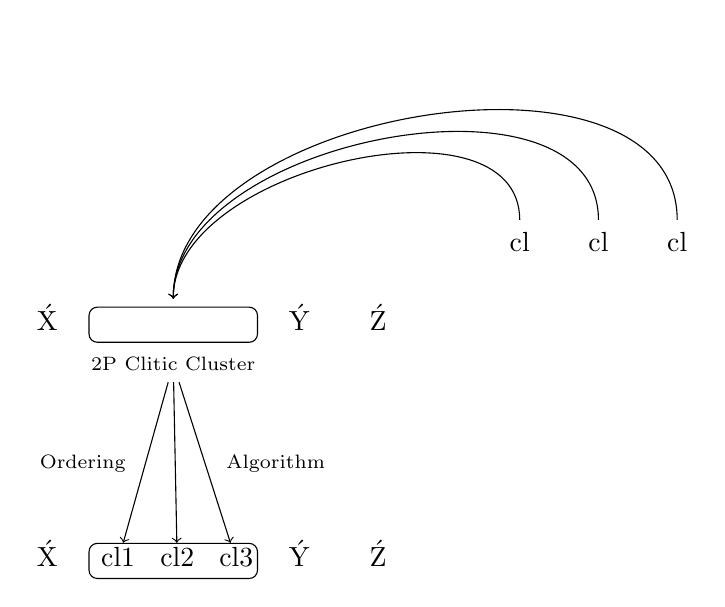
\begin{tikzpicture}[x=1cm,y=1cm,text height=1.2ex, text depth=0.2ex,line/.style={->,shorten >=0.1cm,shorten <=0.1cm}]
\node (cl1) at (6,4) {cl};
\node (cl2) at (7,4) {cl};
\node (cl3) at (8,4) {cl};

\node (X) at (0,3) {\'{X}};
\node[rounded corners=3pt, draw] (rect) at (1.6,3) {\hspace{.75in} }; 
\node (2Pcc) at (1.6,2.5) {{\scriptsize 2P Clitic Cluster}};
\node (Y) at (3.2,3) {\'{Y}};
\node (Z) at (4.2,3) {\'{Z}};
\path [black,line,in=90,out=90] (cl1) edge (rect);
\path [black,line,in=90,out=90] (cl2) edge (rect);
\path [black,line,in=90,out=90] (cl3) edge (rect);

\node (X2) at (0,0) {\'{X}};
\node[rounded corners=3pt, draw] (M) at (1.6,0) {\hspace{.75in} };
\node (Y2) at (3.2,0) {\'{Y}};
\node (Z2) at (4.2,0) {\'{Z}};
\node (cl12) at (.9,0) {cl\sub{1}} ;
\node (cl22) at (1.65,0) {cl\sub{2}};
\node (cl32) at (2.4,0) {cl\sub{3}};

\draw[->] (2Pcc)--(cl12);
\draw[->] (2Pcc)--(cl22);
\draw[->] (2Pcc)--(cl32);

\node (seqq1) at (0.45,1.25) {{\scriptsize Ordering}};
\node (seqq) at (2.9,1.25) {{\scriptsize Algorithm}};
\end{tikzpicture}
\end{center}
\caption{The ``Clitic Cluster''}\label{figure1}
\end{figure}

Typically, the domain\is{clitic!ordering} within which 2P is defined is taken in these approaches to be
prosodically defined, and the entities which undergo 2P placement (the clitics) are taken to be
a prosodic class, but I have never seen an empirically-grounded proposal claiming 
that the observed ordering \textit{within
the \isi{clitic} cluster} is determined by prosodic considerations alone. I imagine that this is because it is pretty hard
to see any trace of the domination of such a factor in the observed \isi{clitic} sequences in these languages.

But in general these authors have not yet ventured a systematic hypothesis about
the sequencing, so it is hard to determine in any detail the nature of the envisioned system.
For example, \citet[108, fn.\ 3]{keydana2011} says ``[a]nother issue not to be
addressed in this paper is the internal structure of \isi{clitic clusters}.'' \citet[88]{goldstein2016} says that because
the matter is a ``difficult issue'', he will ``leave it for future research, and for
the moment assume templatic ordering\ldots ''\footnote{No explicit template is provided which accounts
for the cited data.} \citet[28]{lowe2014}
writes that ``there are regular (though not inviolable) orders when more than one element from
any one of those categories occurs\ldots It is beyond the \isi{scope} of this paper to account for
those patterns.''

Interestingly, each of the authors does seem to feel that the observed ordering is
related to ``classes'' into which the clitics fall. Thirty years ago \citep[73]{hale1987}, I argued that
there were three distinct classes of 2P clitics, taking distinct 2Ps for distinct reasons. 
Although these are not the labels I would use if I were creating them today, and the mechanisms described in 1986
for \textit{how} the categorization of the \isi{clitic} relates to its placement are woefully antiquated,
the classes were: (1) ``emphatic'' clitics, (2) ``sentence connective'' clitics, and (3) ``sentential''
(usually pronominal) clitics. The first I took to involve word-level attachment and the second clause-level. The third
were constrained to appearing in a very low position in what we would now call the CP domain, or,
indeed, at the top of the IP domain. 

I wrote then that ``[t]he position of these elements relative to one
another follows naturally from this account of their origins: the regular sequence is emphatic $+$ 
sentence connective $+$ sentential\ldots '' It is hard to see this statement as anything more than 
either wishful thinking or blissful ignorance, both of which I possessed in spades back in those
days. From my crankier contemporary perspective, it is pretty easy to see that no explicit 
characterization of the membership in
these classes was provided (though I gave isolated examples of each), nor was any mechanism even 
hinted at for what might trigger any
specific ordering in cases of multiple instantiations of one of these categories in a single
clause. In these matters, unfortunately,
I have been largely followed by more recent work. 

I think it is clear enough, however, what we would all like to see. Overt stipulation
is in essence an admission of explanatory failure, and all principles of the scientific pursuit
demand of us that we attempt to minimize the role of stipulation in our models. So, our hope must be that the clitics 
fall into non-arbitrarily-defined classes, and that these \isi{clitic} classes occupy 
well-motivated positions (relative to the functions the clitics instantiate) in the linguistic representation.
Since it is safe to assume that no two clitics do exactly the same work and co-occur in
a single clause, if order falls out in some way from function, we should always be able to generate
a predicted ordering for any pair of clitics. It is the ``in some way'' that I want
to explore today. As a step in that direction, though, I must dwell a little longer on previous work.%\done\todo{check clearpage}
%\clearpage

\section{The Hock template}

Around the same time as I was writing the account discussed above, Hans Hock was
working out the details of an overtly ``templatic'' approach to \isi{clitic} sequencing in \ili{Vedic} \ili{Sanskrit} (e.g.,
\citealt{hock1996}, with earlier literature).\is{templates|(} 
The Hock system was not a model of internal consistency. In this system, the 2P clitics fall into three
classes, P, \'{P}, and {D}: 

\begin{exe}
\ex \begin{tabular}[t]{ll}
P: &  atonic non-``deictic'' (i.e., non-pronominal) clitics\\
\'{P}: & tonic non-``deictic'' clitics (sometimes called ``postpositives'')\\
D: & atonic ``deictics'' (i.e., pronominal clitics)\\
\end{tabular}
\end{exe}

\noindent Clearly, the classification is based on \textit{both} prosodic (tonic vs.\ atonic) and functional considerations\is{prosody}
(deictic vs.\ non-deictic). The template is basically stipulative, but in its most common instantiation, shown in (\ref{ex:hocktemplate}), it is supposed to be 
partially motivated: non-deictics precede deictics (thus P, \'{P} before D, \'{D})
and atonic elements from
each class precede the corresponding tonic elements (thus P before \'{P}, D before \'{D}).

\begin{exe}
	\ex\label{ex:hocktemplate}\'{X}\hspace{.25in}P\hspace{.25in}\'{P}\hspace{.25in}D\hspace{.25in}\'{D}\hspace{.25in}\ldots\
\end{exe}

\noindent The template is often described as ``phonological''
or ``prosodic'' (including by Hock himself), but that, of course, is not accurate. It is important to note that no motivation is cited for either of the two ordering\is{clitics!ordering}
principles: no reason for why non-deictics should come earlier in the clause than the deictics
is given, nor for why the atonic element of each category should precede the tonic one.\footnote{In fact,
\'{D} elements may appear in the \'{X} position and, for Hock's version of the Rigvedic\is{Rigveda} template,
also in the \'{P} position, and thus come earlier in the clause than D elements,
indicating that there isn't much content to this latter principle in
any event.}

The graphical representation of the template in (\ref{ex:hocktemplate}), especially when coupled with the
claim that the template is ``prosodic'', invites the inference that the ``goal'' of the system is have an alternating
strong vs.\ weak tonicity sequence. But since P, \'{P} and D can all double, and since any of those elements can
be absent in any given clause, no such alternating pattern is observed in the vast majority of utterances
in the actual corpus. The prosodic motivation for the template is thus highly abstract (not that that determines\is{prosody}
whether it is accurate or not).

My actual point in discussing the Hock system, however, is to point out that the mechanisms involved are quite distinct from that which we saw in
our discussion of ``\isi{clitic cluster}'' approaches to \isi{clitic} sequencing. We can visualize the system as
seen in Figure~\ref{Halefigure2} below.%\todo{check need for clearpage}
%\clearpage

\begin{figure}%[hbt]
\begin{center}
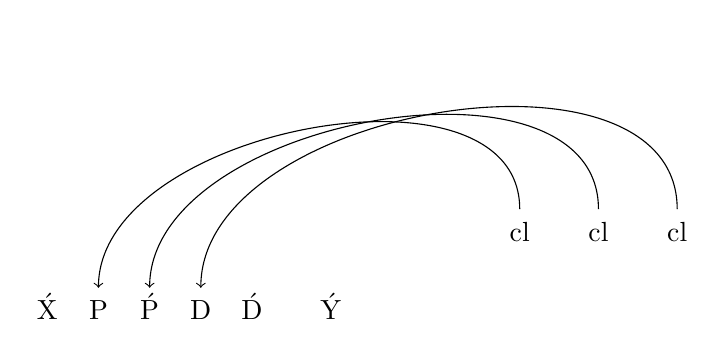
\begin{tikzpicture}[x=1cm,y=1cm,text height=1.2ex, text depth=0.2ex,line/.style={->,shorten >=0.1cm,shorten <=0.1cm}]
\node (cl1) at (6,4) {cl};
\node (cl2) at (7,4) {cl};
\node (cl3) at (8,4) {cl};

\node (X) at (0,3) {\'{X}};
\node (P1) at (.65,3) {P};
\node (P2) at (1.3,3) {\'{P}};
\node (D) at (1.95,3) {D};
\node (Y) at (2.6,3) {\'{D}};
\node (Z) at (3.6,3) {\'{Y}};
\path [black,line,in=90,out=90] (cl1) edge (P1);
\path [black,line,in=90,out=90] (cl2) edge (P2);
\path [black,line,in=90,out=90] (cl3) edge (D);
\end{tikzpicture}
\end{center}
\caption{The ``Hock template''}\label{Halefigure2}
\end{figure}

There is no ``\isi{second position}'' in this conception of things, but a variety of ordered
positions into which clitics are placed based on their properties (prosodic and functional). We can
see the differences between the two general models if we imagine a clause with only a single 2P \isi{clitic}
in it. In the ``\isi{clitic cluster}'' approach that \isi{clitic} will be ``in 2P'', plain and simple. The ordering
algorithm will have no work to do. In an approach such as that found in the Hock template, we can
(and must) still ask the question: where is the \isi{clitic}? It could be in P (with \'{P} and D empty),
or in \'{P} (with P and D empty), or in D (with P and \'{P} empty).

There is, of course, an inherent advantage, given that we are seeking to develop a non-stipulative account
of ordering, if we assume that specific clitics map consistently to specific positions in the
string, and that whether that position ends up being ``second'' or ``third'' or ``fourth'' is simply
the epiphenomenal by-product of the mapping algorithm. A model which, by contrast, dumps the
clitics unordered into a 2P cluster and then must impose an order on them has, in some sense,
missed a chance to impose that ordering earlier in the initial mapping. Particularly if that
mapping is prosody-driven, only a general slackening of constraints on the relationship between
position (at the point of insertion) and interpretation -- constraints which seem to hold of the linguistic
representation generally -- can allow a set of unordered elements, placed by a prosodic algorithm,
to be realigned in an interpretationally-relevant manner (i.e., on the basis of the ``functional
class'' of the \isi{clitic}).

\citet{hale1996} represents an attempt to link the ``positions'' in the Hock template
to specific structural elements within the clause (a similar orientation is found in other
syntax-centric but prosody-sensitive approaches). I will not dwell on that reinterpretation
of Hock here, but instead turn to one more modern model of 2P placement.\is{template|)}

\section{Wackernagel's optimality-theoretic approach}
Wackernagel himself pretty clearly conceived of the 2P phenomenon as a kind of
a compromise between a \isi{clitic} element representing the kind of information which should come
early in the clause (generally because of its ``linking'' function to the preceding context)
and that same element being atonic, and thus not particularly suitable for \isi{initial position}.
This traditional conception is very closely followed by modern Optimality Theoretic approaches
to 2P placement, as reflected, for example, in \citet{anderson2005}.\is{Optimality Theory}

The basic idea of such approaches, as with Wackernagel's, is that there is
a drive for 2P clitics to be initial (captured by an \textsc{AlignLeft} constraint,\is{constraint} which
incurs one violation for each step away from the left edge a \isi{clitic} is) and a prohibition
against the \isi{clitic} appearing in \isi{initial position} (captured by a \textsc{NonInitial} constraint).\is{constraint}
Obviously, both of these constraints cannot be satisfied in the same string. As always
in OT, the conflicting demands are resolved via a \isi{ranking} of the \isi{constraints}.\is{constraint} As long as
\textsc{NonInitial} outranks \textsc{AlignLeft}, the \isi{clitic} will appear \textit{as close
as possible} to string-\isi{initial position}, but not \textit{in} \isi{initial position} -- hence
the 2P effect.

We can see this with a tableau fragment concerning the positioning of Greek \textit{gár} `because,
since' relative to two tonic lexical items, which I designate simply as \'{X} and \'{Y}. Greek
\textit{gár} is a standard example of a ``\isi{Wackernagel's Law}'' element in the language.\footnote{The
reader will notice that this tableau fragment does not select between two ``winning'' outputs:
\'{X} \textit{gár} \'{Y} and \'{Y} \textit{gár} \'{X}. Obviously other constraints will determine
the ultimate optimal output form with respect to the relative ordering of the tonic elements to
one another.}

\begin{exe}
\ex\begin{tabular}[t]{|ll||c|c|}
\firsthline
a. & \'{X}, \'{Y}, gár & \textsc{NonInitial} & \textsc{AlignLeft}(gár) \\ \hline\hline
b. & \'{X} \'{Y} gár &  & \cellcolor{lightgray}*!* \\\hline
c. & \'{X} gár \'{Y} &  & * \\\hline
d. & gár \'{X} \'{Y} & \cellcolor{lightgray}*! & \cellcolor{lightgray} \\\hline
e. & gár \'{Y} \'{X} & \cellcolor{lightgray}*! & \cellcolor{lightgray} \\\hline
f. & \'{Y} gár \'{X} &  & * \\\hline
g. & \'{Y} \'{X} gár &  & \cellcolor{lightgray}*!* \\\hline
\end{tabular}
%\end{center}
%\end{table}
\end{exe}

Wackernagel believed that the drive towards \isi{initial position} was of different
strength for different en\isi{clitic} objects. As long as we make the \textsc{AlignLeft} \isi{constraints}\is{constraint}
\isi{clitic} (or \isi{clitic} class) specific, a strict \isi{ranking} version of OT will require us to decide
for each \isi{clitic} just how strong the demand is that it be aligned left. For example, if we
take the Greek \isi{focus}-marking en\isi{clitic} \textit{mén,} we are \textit{compelled by the model} to ask: is it more
important for \textit{mén} to be on the left, or for \textit{gár} to be on the left? (In Wackernagel's terms,
is the ``drive for \isi{initial position}'' stronger for \textit{mén} or for \textit{gár}?)

The tableau in (\ref{gartab}) below shows how such a system generates -- again by necessity -- a
sequencing of clitics. We should always be attentive, I think, when our modern models seem to converge
on the ideas of important scholars like Wackernagel, who could not have envisioned the workings
of OT, and thus independently had a similar conception of a certain class of linguistic phenomena.
If Wackernagel and Anderson agree, it would be wise to not dissent too quickly!
But is OT the happy confirmation of Wackernagel's less formal and more intuitive analysis?

The model in some sense combines properties of the two earlier approaches I sketched: there
is a sense of a ``fixed stipulative order'' (as seen in the Hock Template) in the relative rankings of
the \textsc{AlignLeft}(x) constraints,\is{constraint} but there is no sense of fixed stipulative positions in the
resulting representation (as that model implies), thus making it more like the ``\isi{clitic cluster}''
analysis. It has the advantage, over the ``\isi{clitic cluster}'' analysis, of not adding a new object
to our model of the grammar (the ``\isi{clitic cluster}''), nor requiring a distinct computational
process which is responsible for explicitly ordering the elements within the cluster (the ``ordering
algorithm'' mentioned above).

\begin{exe}\ex\label{gartab}\begin{tabular}[t]{|lrl||c|c|c|} \firsthline
&&\multirow{2}*{\'{X}, \'{Y}, gár, mén} & \textsc{NonInitial} & \textsc{AlignLeft} & \textsc{AlignLeft} \\ 
&&& \textsc{(cl)} & (mén) & (gár)\\\hline\hline
a. & & \'{X} \'{Y} gár mén &  & \cellcolor{lightgray}**!* & \cellcolor{lightgray}** \\\hline
b. & & \'{X} \'{Y} mén gár &  & \cellcolor{lightgray}**! & \cellcolor{lightgray}*** \\\hline
c. & & \'{X} mén \'{Y} gár &  & * & \cellcolor{lightgray}***! \\\hline
d. & & mén \'{X} \'{Y} gár & \cellcolor{lightgray}*! & \cellcolor{lightgray} & \cellcolor{lightgray}*** \\\hline
e. & & \'{X} gár \'{Y} mén &  & \cellcolor{lightgray}**!* & \cellcolor{lightgray}* \\\hline
f. & & \'{X} gár mén \'{Y} &  & \cellcolor{lightgray}**! & \cellcolor{lightgray}* \\\hline
g. & \hand & \'{X} mén gár \'{Y} &  & * & ** \\\hline
h. & & mén \'{X} gár \'{Y} & \cellcolor{lightgray}*! & \cellcolor{lightgray} & \cellcolor{lightgray}** \\\hline
i. & & gár \'{X} \'{Y} mén & \cellcolor{lightgray}*! & \cellcolor{lightgray}*** & \cellcolor{lightgray} \\\hline
j. & & gár \'{X} mén \'{Y} & \cellcolor{lightgray}*! & \cellcolor{lightgray}** & \cellcolor{lightgray} \\\hline
k. & & gár mén \'{X} \'{Y} & \cellcolor{lightgray}*! & \cellcolor{lightgray}* &\cellcolor{lightgray}  \\\hline
l. & & mén gár \'{X} \'{Y} & \cellcolor{lightgray}*! & \cellcolor{lightgray} & \cellcolor{lightgray}* \\\hline
m. & & gár \'{Y} \'{X} mén & \cellcolor{lightgray}*! & \cellcolor{lightgray}*** & \cellcolor{lightgray} \\\hline
n. & & gár \'{Y} mén \'{X} & \cellcolor{lightgray}*! & \cellcolor{lightgray}** & \cellcolor{lightgray} \\\hline
o. & & gár mén \'{Y} \'{X} & \cellcolor{lightgray}*! & \cellcolor{lightgray}* & \cellcolor{lightgray} \\\hline
p. & & mén gár \'{Y} \'{X} &\cellcolor{lightgray} *! & \cellcolor{lightgray} & \cellcolor{lightgray}* \\\hline
q. & & \'{Y} gár \'{X} mén &  & \cellcolor{lightgray}**!* & \cellcolor{lightgray}* \\\hline
r. & & \'{Y} gár mén \'{X} &  & \cellcolor{lightgray}**! & \cellcolor{lightgray}* \\\hline
s. & \hand & \'{Y} mén gár \'{X} &  & * & ** \\\hline
t. & & mén \'{Y} gár \'{X} & \cellcolor{lightgray}*! & \cellcolor{lightgray} & \cellcolor{lightgray}** \\\hline
u. & & \'{Y} \'{X} gár mén &  & \cellcolor{lightgray}**!* & \cellcolor{lightgray}** \\\hline
v. & & \'{Y} \'{X} mén gár &  & \cellcolor{lightgray}**! & \cellcolor{lightgray}*** \\\hline
w. & & \'{Y} mén \'{X} gár &  & * & \cellcolor{lightgray}***! \\\hline
x. & & mén \'{Y} \'{X} gár & \cellcolor{lightgray}*! & \cellcolor{lightgray}  & \cellcolor{lightgray}*** \\\hline
\end{tabular}
%\end{center}
%\caption{}\end{table}
\end{exe}



I have both conceptual and empirical concerns about the model. At the conceptual level,
stipulation is built into the model pretty deeply: the so-called ``factorial \isi{typology}'' argument
says that we could just as easily have \textsc{AlignLeft}(gár) outrank \textsc{AlignLeft}(mén), and
indeed that every ordering of every available \textsc{AlignLeft}(x) \isi{constraint} should be, in principle,
observed. This does not seem to me to be very consistent with the data I have seen from \isi{archaic \ili{Indo-European} languages} (which often involves etymologically unconnected, but functionally similar enclitics showing
the same ordering principles).

Empirically, one of the great challenges to this model holds, in my view, for all of the
other models we have treated to this point as well. The domain over which the \textsc{AlignLeft}(x) \isi{constraint}
must be assessed is, in the model, a pure stipulation (i.e., there are no principles regulating what
a given en\isi{clitic} might be ``aligned'' to). 
The same problem, in my view, plagues the so-called ``prosody-centric'' approaches which have
become popular: the \isi{clitic} is said to move into the ``\isi{clitic cluster}'' in \isi{second position} of some domain,
but none of the approaches I have seen \citep{keydana2011,lowe2014,goldstein2016} present a non-stipulative characterization
of how the appropriate domain is established. A \isi{clitic} is said to take 2P within (some) \isi{Intonational Phrase},
but the question of which one (when there are multiple IPs in the string) is left unclear. It also seems like the ``Intonational Phrase'' portion of
the specification (and, in non-OT approaches, the 2P part as well) is purely stipulative: could one place a clause-conjoining
\isi{clitic} in 2P of (some) \isi{Utterance Group} or (some) Phonological Word? How about in 3P in the Intonational
Phrase? The models proposed are so inexplicit it is difficult to determine precisely what their allowable
elements and operations are -- the models are thus both highly stipulative and poorly constrained.

As mentioned above, my concerns about the Hock Template have been spelt out in considerable detail in \citet{hale1996},
where I attempt to reduce the empirically valid aspects of the template to the interaction of (1) normal
syntactic placement of the relevant entities and (2) Halpern's \citeyearpar{halpern1995} ``prosodic inversion''. I won't go
through these details here, except to note that in this conception of things en\isi{clitic} elements can be in a variety of structural positions (in the syntax) and may
(or may not) undergo ``prosodic movement''\is{movement} in the \isi{phonology} (depending on whether they are ``properly hosted''
without such movement).

It is obvious that a system which leverages both syntax and phonology to account for
observed \isi{clitic} placement is in some sense more complex than either a purely syntactic or a purely
phonological one.  But the evidence that the process is not \textit{purely syntactic} is, as far as I
can tell, universally accepted. The 2P clitics often interrupt manifest \isi{syntactic constituents} (in
a manner the syntax does not allow) and are quite regularly placed in positions in the string from
which appropriate \isi{scope} relations could not possibly be established. ``Prosodic'' rearrangement
allows the syntax to be mundane rather than strikingly bizarre (with all of the implications 
such bizarreness would have, if allowed, for our theories of grammar).\is{prosody}

That the syntax is involved is, in my view, absolutely required if we are to solve
the ``domain'' problem. \ili{Sanskrit} \textit{ca} and Attic \textit{te} are 2P clitics, but they appear
in clause-\isi{second position} only when their domain is the clause. They appear in ``DP-second'' position
when their domain is the DP, and in VP-\isi{second position} when their domain is the VP. Their domain
simply cannot be defined with respect to \textit{prosody} alone.

\section{Sample application: En\isi{clitic} subordination}
\is{subordination|(}Both of these observations can be seen to be at work in a set of examples involving
en\isi{clitic} subordinators. Before examining this data, which will also display the mechanisms I believe
are at work in \isi{clitic} placement (and thus what we might use to explain \isi{clitic} sequencing), I will
remind the reader that \citet{hale1987} showed that there was a process manifest in the language of
the \isi{Rigveda}, in \isi{Avestan}, and in Greek, whereby a single constituent could be fronted to the left
of a WH-element. Obviously, this analysis extends (though the matter was not overtly discussed -- but rather
implicitly assumed -- in
that earlier work) to other subordinators present in C (`if', `when', `because'). I will call that \isi{fronting}
process ``\isi{topicalization}'' (and the position into which the \isi{fronting} takes place Top), with no
particular commitment to the \isi{discourse} functions involved.

Familiar examples of this \isi{fronting} looks like this:

%\pex\label{Top}
%\a
%\begingl[glhangstyle=none,everygla=\it,everyglb=,everyglft=\rm]
%\gla {[}áśmānam cid] yé bibhidúr vácobhiḥ //
%\glb rock-ASg Emph.\textit{cl} Rel-NPlM smashed-IIIPl words-ISgN //
%\glft `who smashed even rock with (mere) words\ldots ' \trailingcitation{RV 4.16.6c} //
%\endgl
%\a
%\begingl[glhangstyle=none,everygla=\it,everyglb=,everyglft=\rm]
%\gla {[}idhmáṃ] yás te jabhárac chaśramāṇáḥ //
%\glb kindling-ASg Rel-NSg you-DSg.\textit{cl} {would bear-IIISg} {exerting himself-NSg} //
%\glft `who, exerting himself, would bear the kindling to you\ldots ' \trailingcitation{RV 4.12.2a} //
%\endgl
%\xe

\begin{exe}
\ex\label{Top}
	\begin{xlist}
	\ex
		\gll {\ob}áśmānam cid{\cb} yé bibhidúr vácobhiḥ \\
			{\db}rock-Asg Emph.\textit{cl} Rel-NPlM smashed-IIIPl words-ISgN \\
		\glt `who smashed even rock with (mere) words\ldots{}' \hfill {RV 4.16.6c}
	\ex
		\gll {\ob}idhmáṃ{\cb} yás te jabhárac \\
			{\db}kindling-ASg Rel-NSg you-DSg.\textit{cl} {would bear-IIISg} \\
		
		\gll \hspace*{1em} chaśramāṇáḥ \\
			{} {exerting himself-NSg} \\
		\glt `who, exerting himself, would bear the kindling to you\ldots{}' \hfill {RV 4.12.2a}
	\end{xlist}
\end{exe}

\noindent Armed with the following assumptions, then, let us see what some structures look like, and how they might impact the development of a theory of \isi{clitic} sequencing:

\begin{itemize}
\item en\isi{clitic} elements are placed in ``expected'' syntactic position
\item ``prosodic inversion'' is triggered when they are not properly hosted on their left edge
\end{itemize}

Wackernagel proposed long ago that there were traces in the \isi{Rigveda} of a reflex
of IE \textit{*kʷe} which (like OLat.\ \textit{absque me esset} `if it were
without me', some uses of Gothic \textit{nih}, and, although not known to \isi{Wackernagel},
\ili{Hittite} \textit{takku}) is subordinating in function, generally rendered `if, when.'
As might be expected, the verb in such clauses, as in subordinate clauses in
\ili{Vedic} generally, is accented. This has given rise to some anxiety that the true
subordination marker is the verbal accent, and that \textit{ca} is simply (weakly)
coordinating. Typical examples are:

%\pex\label{2Psubca}
%\a
%\begingl[glhangstyle=none,everygla=\it,everyglb=,everyglft=\rm]
%\gla níuptāś ca babhrávo vā́cam ákratam̐ + émī́d eṣāṃ niṣkr̥táṃ jāríṇīva //
%\glb scattered-down \textbf{ca} brown-NPl voice-ASg {they made} {I go=PTCL} their$_{cl}$ {appointed place-ASg} {paramour-NSg}=like // 
%\glft `And as soon as, scattered down, the brown (dice) have raised their voice, I just go to their appointed place, like a girl with a lover.' (SJ/JB) \trailingcitation{10.34.5cd} //
%\endgl
%\a
%\begingl[glhangstyle=none,everygla=\it,everyglb=,everyglft=\rm]
%\gla tuváṃ ca soma no váśo + jīvā́tuṃ ná marāmahe //
%\glb you-NSg \textbf{ca} Soma-VSg us$_{cl}$ {you should wish} {to live} \textsc{Neg} {we will die} //
%\glft `And if you will wish us to live, Soma, we will not die.' (SJ/JB) \trailingcitation{RV 1.91.6ab} //
%\endgl
%\xe

\begin{exe}
\ex\label{2Psubca}
	\begin{xlist}
	\ex\gll níuptāś ca babhrávo vā́cam ákratam̐ \\
			scattered-down \textbf{ca} brown-NPl voice-ASg {they made}\\
			
		\gll émī́d eṣāṃ niṣkr̥táṃ jāríṇīva \\
			 {I go=PTCL} their\subit{cl} {appointed place-ASg} {paramour-NSg}=like \\
		\glt `And as soon as, scattered down, the brown (dice) have raised their voice, I just go to their appointed place, like a girl with a lover.' (SJ/JB)		\hfill {10.34.5cd}
	\ex\gll tuváṃ ca soma no váśo\\
			you-NSg \textbf{ca} Soma-VSg us\subit{cl} {you should wish}\\

		\gll jīvā́tuṃ ná marāmahe \\
			 {to live} \textsc{Neg} {we will die} \\
		\glt `And if you will wish us to live, Soma, we will not die.' (SJ/JB)		\hfill {RV 1.91.6ab}
	\end{xlist}
\end{exe}

\noindent I have provided the translation of \citet{jamison2014} because it reflects directly the unease
that some Vedicists feel about ``subordinating'' \textit{ca}: they have translated `and as soon as (=when)' and
`and if', leaving
it unclear whether they believe that \textit{ca} is coordinating (`and') and the verbal accent
subordinating (`as soon as', `if'), or whether perhaps they believe that this \textit{ca} actually means `and as soon as/if'.

As one can imagine, determining whether or not such clauses are weakly connected to the preceding
\isi{discourse} -- i.e., whether the `and' should be in the \ili{English} translation -- is no easy task. And from
this example, and other widely accepted ones (such as RV 8.21.6ab below), in which \textit{ca} occupies
\isi{second position}, it doesn't seem likely that our approach to clitics is going to be much help
in this task.

%\ex
%\begingl[glhangstyle=none,everygla=\it,everyglb=,everyglft=\rm]
%\gla áchā ca tvainā́ námasā vádāmasi + kím múhuś cid ví dīdhayaḥ //
%\glb PV \textbf{ca} you$_{cl}$=this-ISg homage-ISg {we address} Q-marker {for a moment} even$_{cl}$ PV {you will think} //
%\glft `When we address you with this homage, will you hesitate even for a moment?'  \trailingcitation{RV 8.21.6ab} //
%\endgl
%\xe

\begin{exe}
\ex\gll áchā ca tvainā́ námasā vádāmasi \\
		PV \textbf{ca} you\subit{cl}=this-ISg homage-ISg {we address} \\
		
	\gll kím múhuś cid ví dīdhayaḥ \\
		Q-marker {for a moment} even\subit{cl} PV {you will think} \\
	\glt `When we address you with this homage, will you hesitate even for a moment?'
	
	{ }\hfill {RV 8.21.6ab}
\end{exe}

\noindent Hettrich \citeyearpar[252]{hettrich1988} notes overtly  on subordinating \textit{ca} that \textit{ca} stands ``wie nach Wackernagels 
Enklisengesetz[fn deleted] zu erwarten, überwiegend an zweiter Stelle im Satz.''\footnote{`\ldots as would be expected
according to \isi{Wackernagel's Law}, overwhelmingly in the \isi{second position} in the clause.'}

It is somewhat striking to see the \textit{überwiegend} in this statement, because coordinating
\textit{ca} is extremely regular in its ``\isi{second position}'' behavior, being postponed only in cases
in which there is a ``\isi{phonological word}'' at the start of the conjoined domain. Are there actually cases
of ``late \textit{ca}'' in subordinating function? The following examples seem to answer this question
``yes''.

%\pex\label{lateca}
%\a
%\begingl[glhangstyle=none,everygla=\it,everyglb=,everyglft=\rm]
%\gla asyá ślóko divī́yate pr̥thivyā́m + átyo ná yaṃsad yakṣabhŕ̥d vícetāḥ + mr̥gā́ṇāṃ ná hetáyo yánti cemā́ + bŕ̥haspáter áhimāyām̐ abhí dyū́n //
%\glb his call-NSg heaven-LSg=speeds earth-LSg steed-NSg like {will control} bringing-wondrous-apparitions-NSg discriminating-NSg {wild beasts-GPl} like charges-NPl {they go} \textbf{ca}=these-NPl Brhaspati-GSg having-snake-wiles-APl to heavens-APl //
%\glft `The discriminating one [=Br̥haspati?], like a steed, bringing wondrous apparitions, will control it when these (words) of Brhaspati, like the charges of wild beasts, go to the snake-wiles-possessing heavens.' \trailingcitation{RV 1.190.4} //
%\endgl
%\a
%\begingl[glhangstyle=none,everygla=\it,everyglb=,everyglft=\rm]
%\gla ubháyaṃ śr̥ṇávac ca na + índro arvā́g idáṃ vácaḥ + satrā́ciyā maghávā sómapītaye + dhiyā́ śáviṣṭha ā́ gamat //
%\glb twofold-ASg {will hear} \textbf{ca} us$_{cl}$ Indra-NSg nearby this-ASg speech-ASg fully-focussed-ISg benefactor-NSg soma-drinking-DSg thinking-ISg most-powerful-NSg PV {will come} //
%\glft `When Indra nearby will hear this twofold speech of ours, the most powerful benefactor will come here to the soma-drinking by reason of our fully focussed insight.' \trailingcitation{RV 8.61.1} //
%\endgl
%\xe

\begin{exe}
\ex\label{lateca}
	\begin{xlist}
	\ex\gll asyá ślóko divī́yate pr̥thivyā́m \\
			his call-NSg heaven-LSg=speeds earth-LSg \\
			
		\gll átyo ná yaṃsad yakṣabhŕ̥d \\
			steed-NSg like {will control} bringing-wondrous-apparitions-NSg \\
			
		\gll \hspace*{1em} vícetāḥ \\
			{} discriminating-NSg \\
			
		\gll mr̥gā́ṇāṃ ná hetáyo yánti cemā́ \\
			{wild beasts-GPl} like charges-NPl {they go} \textbf{ca}=these-NPl \\
		\gll bŕ̥haspáter áhimāyām̐ abhí dyū́n \\
			Brhaspati-GSg having-snake-wiles-APl to heavens-APl \\
		\glt `The discriminating one [=Br̥haspati?], like a steed, bringing wondrous apparitions, will control it when these (words) of Brhaspati, like the charges of wild beasts, go to the snake-wiles-possessing heavens.'		\hfill {RV 1.190.4}
	\ex\gll ubháyaṃ śr̥ṇávac ca na \\
		twofold-ASg {will hear} \textbf{ca} us\subit{cl} \\
		
		\gll índro arvā́g idáṃ vácaḥ \\
		Indra-NSg nearby this-ASg speech-ASg \\
		
		\gll satrā́ciyā maghávā sómapītaye \\
			fully-focussed-ISg benefactor-NSg soma-drinking-DSg \\
			
		\gll dhiyā́ śáviṣṭha ā́ gamat \\
			thinking-ISg most-powerful-NSg PV {will come} \\
		\glt `When Indra nearby will hear this twofold speech of ours, the most powerful benefactor will come here to the soma-drinking by reason of our fully focussed insight.' \hfill {RV 8.61.1} \\
	\end{xlist}
\end{exe}

\noindent To understand this data (and there are one or two more examples), we need to ask the following question: how does
\isi{conjunctive} \textit{ca} end up in ``\isi{second position}'' when it conjoins clauses, and how would we expect a ``subordinating
\textit{ca}'' to behave given the assumptions outlined above?

The behavior of coordinating \textit{ca} is fairly straightforward. No matter what kind of syntactic (or prosodic!)
entity \textit{ca} is coordinating,
it appears in this configuration:

\begin{exe}
\ex\begin{forest}
	[XP
		[\textit{ca}]
		[XP
			[{X Y Z}, roof]
		]
	]
\end{forest}
\end{exe}


\noindent {\ob}X Y Z{\cb} can be a clause, as in the case under discussion, or an DP or VP or PP or whatever. Obviously, \textit{ca} sits
at the left edge of the XP-domain and thus does not have a proper prosodic host to its left. It therefore must undergo
the ``prosodic flip'', and, assuming X is a ``\isi{phonological word}'', the resulting operation will give rise to this
string:

\begin{exe}
	\ex
%\begin{center}
{\textcolor{gray}{{\rnode{A}{\textit{ca}}}} X {\rnode{B}{\textit{ca}}}} Y Z \ncarc[arcangle=270,nodesep=3pt]{<-}{B}{A}
%
%\end{center}
\end{exe}

\noindent It should be clear that one thing that \textit{ca} can bring into a \isi{coordination} relationship with what precedes it
is a clause introduced by a \textit{topicalized} phrase. Here's an example.

%\ex
%\begingl[glhangstyle=none,everygla=\it,everyglb=,everyglft=\rm]
%\gla yád agna eṣā́ sámitir bhávāti + devī́ devéṣu yajatā́ yajatra + rátnā ca yád vibhájāsi svadhāvo + bhāgáṃ no átra vásumantaṃ vītāt //
%\glb when Agni-VSg this-NSg assembly-NSg {will become} godly-NSg gods-LPl sacrifical-NSg {sacrificial one} treasures-APl and$_{cl}$ when {you will share out} having-independent-will-VSg share-ASg us$_{cl}$ then rich-in-goods-ASg pursue //
%\glft `When, o Agni, this assembly will become godly among the gods, a sacrificial one, o sacrificial one, and when you will share out treasures, o you of independent will, then pursue a share for us rich in goods.' (SJ/JB) \trailingcitation{RV 10.11.8} //
%\endgl
%\xe

\begin{exe}
\ex\gll yád agna eṣā́ sámitir bhávāti \\
	when Agni-VSg this-NSg assembly-NSg {will become} \\
	
	\gll devī́ devéṣu yajatā́ yajatra \\
	godly-NSg gods-LPl sacrifical-NSg {sacrificial one} \\
	
	\gll rátnā ca yád vibhájāsi \\
	treasures-APl and\subit{cl} when {you will share out} \\
	
	\gll \hspace*{1em} svadhāvo \\
		{} having-independent-will-VSg \\
	
	\gll bhāgáṃ no átra vásumantaṃ vītāt \\
	share-ASg us\subit{cl} then rich-in-goods-ASg pursue \\
	\glt `When, o Agni, this assembly will become godly among the gods, a sacrificial one, o sacrificial one, and when you will share out treasures, o you of independent will, then pursue a share for us rich in goods.' (SJ/JB)
	
	\hfill {RV 10.11.8}
\end{exe}

The c-pada of this verse arises from a \textit{syntactic} structure of the form:

\begin{exe}
\ex\label{caTOP} 
\begin{forest}
for tree={fit=band}
[TopP
	[\textit{ca}]
	[TopP
		[\textit{rátnā}]
		[CP
			[\textit{yád}]
			[IP
				[{\textit{vibhájāsi svadhāvo}}, roof]
			]
		]
	]
]
\end{forest}
\end{exe}

%\ex\label{caTOP} 
%
%\Tree [.TopP \textit{ca} [.TopP \textit{rátnā} [.CP  \textit{yád} \qroof{\textit{vibhájāsi svadhāvo}}.IP ] ] ] 
%
%\xe

So where do we expect \textbf{subordinating} \textit{ca} to be \textit{syntactically}? Well, it is \textit{isofunctional}
with \textit{yád} in the clause above. So the structure of the subordinate clause in
(\ref{2Psubca}a) at the end of \textit{syntactic} computation
would presumably be:

%\ex
%
%\Tree [.CP \textit{ca} \qroof{[\textit{níuptās babhrávas}] \textit{vā́cam ákrata}}.IP ]
%
%\xe

\begin{exe}
\ex\begin{forest}
[CP
	[\textit{ca}, fit=band]
	[IP
		[{[\textit{níuptās babhrávas}] \textit{vā́cam ákrata}}, roof]
	]
]
\end{forest}
\end{exe}

\noindent Since \textit{ca} is alone up there in the left periphery, it must undergo the ``prosodic flip'' in the phonology
to be properly hosted.


What would happen if we were to have a Top element in such a clause? In the case of \isi{coordination}, it of
course is the entire clause, including its initial Topic-phrase, which gets coordinated to a preceding (or following) clause, and \textit{ca} thus
dominates TopP. But topicalized material appears to the \textit{left} of the subordinator (relative pronouns,
\textit{yádi} `if', etc.), so if \textit{ca} is a subordinator, we predict a structure such as (contrast coordinating
\textit{ca}
in (\ref{caTOP})):\is{subordination}

%\ex
%
%\Tree [.TopP Topic [.CP \textit{ca} \qroof{X Y Z}.IP ] ]
%
%\xe

\begin{exe}
\ex\begin{forest}
for tree={fit=band}
[TopP
	[Topic]
	[CP
		[\textit{ca}]
		[IP
			[{X Y Z}, roof]
		]
	]
]
\end{forest}
\end{exe}

If the proper ``hosting domain'' for \textit{ca} is the CP, then it is unhosted on its left, and we predict the
\textit{phonology} to restructure this to:

\begin{exe}
	\ex
%\begin{center}
Topic {\ob}{\textcolor{gray}{{\rnode{A}{\textit{ca}}}} X {\rnode{B}{\textit{ca}}}} Y Z{\cb} \ncarc[arcangle=270,nodesep=3pt]{<-}{B}{A}
%
%\end{center}
\end{exe}

\noindent Note that, if there are such examples, since coordinating \textit{ca} won't act this way, but subordinating \textit{ca}
should, we would have clear and unambiguous evidence for the \textit{syntactic separation} of \textit{ca} into two distinct
types of grammatical element. And of course there are such examples. We saw them above in (\ref{lateca}ab), whose structures
are:

\begin{exe}
	\ex
	\begin{xlist}
		\ex
%\begin{itemize}
%\item[a.]
{\ob}\sub{Top} \textit{mr̥gā́ṇāṃ ná hetáyo}{\cb} {\ob}\sub{CP} {\textcolor{gray}{\textit{c\rnode{A}a}}} {\ob}\textit{yánti \rnode{B}{ca} imā́ bŕ̥haspáter áhimāyām̐ abhí dyū́n}{\cb}{\cb}\ncarc[arcangle=270,nodesep=3pt]{<-}{B}{A}
\vspace{.11in}

\ex
%\item[b.]
{\ob}\sub{Top} \textit{ubháyaṃ}{\cb} {\ob}\sub{CP} {\textcolor{gray}{\textit{c\rnode{A}a}}} {\ob}\textit{śr̥ṇávac \rnode{B}{ca} na índro arvā́g idáṃ vácaḥ}{\cb}{\cb} \ncarc[arcangle=270,nodesep=3pt]{<-}{B}{A}
%\end{itemize}
\end{xlist}
\end{exe}

The construction as a whole is rare, but confirmation for this analysis is provided by the reflex of subordinating
\textit{ca} in later \ili{Vedic} texts (and, rarely, already in the \isi{Rigveda}) -- the subordinating particle \textit{céd} (etymologically from \textit{ca} $+$ 
\textit{íd}). The ``normal''
position for this particle is, of course, in \isi{second position}.

%\pex
%\a 
%\begingl[glhangstyle=none,everygla=\it,everyglb=,everyglft=\rm]
%\gla ná vā́ araṇyānír hanti + anyáś cén nā́bhigáchati //
%\glb \textsc{Neg} PTCL {Lady of the Wilderness-NSg} slays another-NSg \textbf{céd} \textsc{Neg}=attacks //
%\glft `In truth, the Lady of the Wilderness does no slaughter, if someone else does not attack.' (SJ/JB) \trailingcitation{RV 10.146.5ab} //
%\endgl
%\a 
%\begingl[glhangstyle=none,everygla=\it,everyglb=,everyglft=\rm]
%\gla yó asyā ū́dho ná veda- + -atho asyā stánān utá + ubháyenaivā́smai duhe + dā́tuṃ céd áśakad vaśā́m //
%\glb who-NSg her-GSg$_{cl}$ udder-ASg \textsc{Neg} knows thereto=PTCL her-GSg$_{cl}$ teats-APl {as well} both-ISg=PTCL=him-DSg$_{cl}$ {she yields milk} {to give} \textbf{céd} {he was able} cow-ASg  //
%\glft `Whoever knows not the udder of her, and likewise the teats of her, to him she yields milk with both, if he has been able to give the cow.' (Whitney) \trailingcitation{AVŚ 12.4.18} //
%\endgl
%\xe

\begin{exe}
\ex
	\begin{xlist}
	\ex\gll ná vā́ araṇyānír hanti \\
			\textsc{Neg} PTCL {Lady of the Wilderness-NSg} slays \\
			
		\gll anyáś cén nā́bhigáchati \\
			another-NSg \textbf{céd} \textsc{Neg}=attacks \\
		\glt `In truth, the Lady of the Wilderness does no slaughter, if someone else does not attack.' (SJ/JB) \hfill {RV 10.146.5ab}
	\ex\gll yó asyā ū́dho ná veda-\\
			who-NSg her-GSg\subit{cl} udder-ASg \textsc{Neg} knows \\
			
		\gll -atho asyā stánān utá \\
			thereto=PTCL her-GSg\subit{cl} teats-APl {as well} \\
			
		\gll ubháyenaivā́smai duhe \\
			both-ISg=PTCL=him-DSg\subit{cl} {she yields milk} \\
			
		\gll dā́tuṃ céd áśakad vaśā́m \\
			{to give} \textbf{céd} {he was able} cow-ASg \\
		\glt `Whoever knows not the udder of her, and likewise the teats of her, to him she yields milk with both, if he has been able to give the cow.' (Whitney) \hfill {AVŚ 12.4.18} \\
	\end{xlist}
\end{exe}

But, as with subordinating \textit{ca}, we find unexpectedly ``late'' instances of \textit{céd} as well.

%\pex
%\a 
%\begingl[glhangstyle=none,everygla=\it,everyglb=,everyglft=\rm]
%\gla {[}arthíno] yánti céd árthaṃ + gáchān íd dadúṣo rātím//
%\glb having-a-task-NPl proceed \textbf{céd} task-ASg {they will go to} PTCL giver-GSg generosity-ASg //
%\glft `If those having a task proceed to their task, they will attain the generosity of the giver.' \trailingcitation{RV 8.79.5ab} //
%\endgl
%\a 
%\begingl[glhangstyle=none,everygla=\it,everyglb=,everyglft=\rm]
%\gla {[}abandhv éke dádataḥ prayáchanto] + dā́tuṃ céc chíkṣānt sá svargá evá //
%\glb kinless-NPl some-NPl giving-NPl bestowing-NPl {to give} \textbf{céd} {they are able} this-NSg heaven-NSg indeed //
%\glft `If some, without kin, giving, bestowing, are able to give, this is truly heaven.' \trailingcitation{AVŚ 6.122.2cd} //
%\endgl
%\a 
%\begingl[glhangstyle=none,everygla=\it,everyglb=,everyglft=\rm]
%\gla héḍaṃ paśūnā́ṃ ny èti + brāhmaṇébhyó 'dadad vaśā́m + [devā́nāṃ níhitaṃ bhāgáṃ] + mártyaś cén nipriyāyáte //
%\glb wrath-ASg cattle-GPl PV comes Brahmans-DPl not-giving-NSg cow-ASg gods-GPl deposited-ASg portion-ASg mortal-NSg \textbf{céd} {keeps (for himself)} //
%\glft `The mortal not giving a cow to the Brahmans goes down to the wrath of the cattle, if he keeps to himself the deposited portion of the gods.' \trailingcitation{AVŚ 12.4.21} //
%\endgl
%\xe

\begin{exe}
\ex
	\begin{xlist}
	\ex\gll {\ob}arthíno{\cb} yánti céd árthaṃ \\
			{\db}having-a-task-NPl proceed \textbf{céd} task-ASg \\
			
		\gll gáchān íd dadúṣo rātím \\
			{they will go to} PTCL giver-GSg generosity-ASg \\
		\glt `If those having a task proceed to their task, they will attain the generosity of the giver.' \hfill \mbox{RV 8.79.5ab}
	\ex\gll {\ob}abandhv éke dádataḥ prayáchanto{\cb} \\
			{\db}kinless-NPl some-NPl giving-NPl bestowing-NPl \\
			
		\gll dā́tuṃ céc chíkṣānt sá svargá evá \\
			{to give} \textbf{céd} {they are able} this-NSg heaven-NSg indeed \\
		\glt `If some, without kin, giving, bestowing, are able to give, this is truly heaven.' \hfill {AVŚ 6.122.2cd}
	\ex\gll héḍaṃ paśūnā́ṃ ny èti \\
			wrath-ASg cattle-GPl PV comes \\
			
		\gll brāhmaṇébhyó 'dadad vaśā́m \\
			Brahmans-DPl not-giving-NSg cow-ASg \\
			
		\gll {\ob}devā́nāṃ níhitaṃ bhāgáṃ{\cb} \\
			{\db}gods-GPl deposited-ASg portion-ASg \\
			
		\gll mártyaś cén nipriyāyáte \\
			mortal-NSg \textbf{céd} {keeps (for himself)} \\
		\glt `The mortal not giving a cow to the Brahmans goes down to the wrath of the cattle, if he keeps to himself the deposited portion of the gods.'
		
		\hfill {AVŚ 12.4.21}
	\end{xlist}
\end{exe}

\noindent And note that we can use our analysis of these ``late'' instances to make our interpretations of certain
\ili{Vedic} passages more precise. Look at the AB passage (from the Śunaḥśepa legend) in (\ref{AB7}).

%\ex\label{AB7}
%\begingl[glhangstyle=none,everygla=\it,everyglb=,everyglft=\rm]
%\gla r̥nam asmin saṃnayaty + amr̥tatvaṃ ca gachati + pitā putrasya jātasya + paśyec cej jīvato mukham //
%\glb debt-ASg him-LSg$_{cl}$ {he pays} immortality-ASg and$_{cl}$ {he goes to} father-NSg son-GSg born-GSg {he should see} \textbf{ced} living-GSg face-ASg //
%\glft `A debt he payeth in him, and immortality he attaineth, that father who seeth the face of a son born living.' (Keith) \trailingcitation{AB 7.13.4} //
%\endgl
%\xe

\begin{exe}
\ex\label{AB7}
	\gll r̥nam asmin saṃnayaty \\
		debt-ASg him-LSg\subit{cl} {he pays} \\
		
	\gll amr̥tatvaṃ ca gachati \\
		immortality-ASg and\subit{cl} {he goes to} \\
		
	\gll pitā putrasya jātasya \\
		father-NSg son-GSg born-GSg \\
		
	\gll paśyec cej jīvato mukham \\
		{he should see} \textbf{ced} living-GSg face-ASg \\
	\glt `A debt he payeth in him, and immortality he attaineth, that father who seeth the face of a son born living.' (Keith) \hfill {AB 7.13.4}
\end{exe}

\noindent Keith, whose translation I have provided, takes {\ob}putrasya jātasya\ldots\ jīvato mukham{\cb} `(the) face of a son born living' as a (discontinuous) constituent, the direct object of the verb \textit{paśyet}. That is, his analysis (ignoring for a moment
the \textit{ced}, to which we will turn momentarily) is that the subject and predicate divide like this:

\begin{exe}
	\ex
%\begin{center}
{\ob}\textit{pitā}{\cb} {\ob}\textit{putrasya jātasya paśyet jīvato mukham}{\cb}
%\end{center}
\end{exe}

\noindent There are two possibilities for where \textit{pitā} could be under Keith's interpretation: it could have been fronted into the Topic position, or,
of course, it could be in some position lower than C (in Focus, or in \textsc{IP}, e.g.). If it were below C, the output
of the syntax (now with \textit{ced} reintroduced) would have been as below, with the ``prosodic flip'' indicated:

%\begin{center}
\vspace*{1ex}
\begin{exe}\ex
{\ob}\sub{CP} {\textcolor{gray}{\textit{c\rnode{A}ed}}} {\ob}\textit{pitā \rnode{B}{ced} putrasya jātasya paśyet jīvataḥ mukham}{\cb}{\cb} \ncarc[arcangle=270,nodesep=3pt]{<-}{B}{A}
\end{exe}
%\end{center}


If \textit{pitā} were in Topic, we would have instead expected:

\vspace*{2ex}
\begin{exe}\ex
%\begin{center}
{\ob}\sub{Topic} \textit{pitā}{\cb} {\ob}\sub{CP} {\textcolor{gray}{\textit{c\rnode{A}ed}}} {\ob}\textit{putrasya \rnode{B}{ced} jātasya paśyet jīvataḥ mukham}{\cb}{\cb} \ncarc[arcangle=270,nodesep=3pt]{<-}{B}{A}
%\end{center}
\end{exe}


\noindent Neither of these is the sentence in the text. It is clear what the structure must be if the placement of \textit{ced}
is to fit with all the other evidence for the use of this particle in early \ili{Vedic}:

\begin{exe}\ex
%\begin{center}
{\ob}\sub{Topic} \textit{pitā putrasya jātasya}{\cb} {\ob}\sub{CP} {\textcolor{gray}{\textit{c\rnode{A}ed}}} {\ob}\textit{paśyet \rnode{B}{ced} jīvataḥ mukham}{\cb}{\cb} \ncarc[arcangle=270,nodesep=3pt]{<-}{B}{A}

`when the father of a (just) born son\subit{i} sees the face of (him\subit{i}) living'
%\end{center}
\end{exe}\is{subordination|)}

\section{\textit{hí}, \textit{gár}, and clitic sequencing}

In my dissertation \citep{hale1987}, I dealt fairly extensively with the data from \ili{Vedic} \textit{hí}
`because, since'. I noted that while the vast majority of instances of \textit{hí} are in ``\isi{second position}'' (appropriately
defined), there were a number of counterexamples. Note that \textit{hí} occupies, at the end of the syntactic computation,
the very same position (``C'') as subordinating \textit{ca} and \textit{céd}.

I won't bother citing \isi{second position} instances of \textit{hí} -- as I said,
the vast majority of the approx.\ 630 attestations of the particle are in that slot, properly defined. Some of the
not terribly numerous exceptions are given in (\ref{hiexc}) below. Several interesting issues arise, so I cite a
healthy number of the exceptions.

%\pex\label{hiexc}
%\a
%\begingl[glhangstyle=none,everygla=\it,everyglb=,everyglft=\rm]
%\gla urukramásya sá hí bándhur itthā́ //
%\glb wide-striding-GSg this-NSg \textbf{hí} bond-NSg thus //
%\glft `for exactly that is the bond to the wide-striding one' (SJ/JB) \trailingcitation{RV 1.154.5c} //
%\endgl
%\a
%\begingl[glhangstyle=none,everygla=\it,everyglb=,everyglft=\rm]
%\gla asmā́ñ ca tā́ṃś ca prá hí néṣi vásya ā́ //
%\glb us-APl and$_{cl}$ them-APl and$_{cl}$ PV \textbf{hí} lead better-ASg PostP //
%\glft `lead both us and them forth to a better state.' (SJ/JB) \trailingcitation{RV 2.1.16c} //
%\endgl
%\a 
%\begingl[glhangstyle=none,everygla=\it,everyglb=,everyglft=\rm]
%\gla tribhíḥ pavítrair ápupod dhí arkáṃ //
%\glb three-IPl purifiers-IPl {he purified} \textbf{hí} chant-ASg //
%\glft  `Since he [=Agni?] purified the chant with three purifying filters,' (SJ/JB) \trailingcitation{RV 3.26.8a} //
%\endgl
%\a 
%\begingl[glhangstyle=none,everygla=\it,everyglb=,everyglft=\rm]
%\gla ákṣetravit kṣetravídaṃ hí áprāṭ //
%\glb not-knowing-the-field-NSg knowing-the-field-ASg \textbf{hí} asked //
%\glft `Because the one not knowing the field asked the field-knower,' (SJ/JB) \trailingcitation{RV 10.32.7a} //
%\endgl
%\xe

\begin{exe}
\ex\label{hiexc}
	\begin{xlist}
	\ex\gll urukramásya sá hí bándhur itthā́ \\
			wide-striding-GSg this-NSg \textbf{hí} bond-NSg thus \\
		\glt `for exactly that is the bond to the wide-striding one' (SJ/JB)
		
		\hfill {RV 1.154.5c}
	\ex\gll asmā́ñ ca tā́ṃś ca prá hí néṣi vásya ā́ \\
			us-APl and\subit{cl} them-APl and\subit{cl} PV \textbf{hí} lead better-ASg PostP \\
		\glt `lead both us and them forth to a better state.' (SJ/JB) \hfill {RV 2.1.16c} 
	\ex\gll tribhíḥ pavítrair ápupod dhí arkáṃ \\
			three-IPl purifiers-IPl {he purified} \textbf{hí} chant-ASg \\
		\glt `Since he [=Agni?] purified the chant with three purifying filters,' (SJ/JB)
		
		\hfill {RV 3.26.8a}
	\ex\gll ákṣetravit kṣetravídaṃ hí áprāṭ \\
			not-knowing-the-field-NSg knowing-the-field-ASg \textbf{hí} asked \\
		\glt `Because the one not knowing the field asked the field-knower,' (SJ/JB)
		
		\hfill {RV 10.32.7a}
	\end{xlist}
\end{exe}

\noindent In all of the ``exceptions'' I will cite here, we can analyze the data just as we did in the case of
\textit{ca} and \textit{céd}: the first constituent of the clause is in the Topic position
above the CP, \textit{hí} is in C itself, and is not ``properly hosted'' by a tonic element \textit{within
its domain} on its left, and thus undergoes inversion. Thus we have {\ob}\sub{Top} \textit{urukramásya}{\cb}
in (\ref{hiexc}a), {\ob}\sub{Top} \textit{asmā́ñ ca tā́ṃś ca}{\cb} in (\ref{hiexc}b), {\ob}\sub{Top} \textit{tribhíḥ pavítrair}{\cb}
in (\ref{hiexc}c), and {\ob}\sub{Top} \textit{ákṣetravit}{\cb} in (\ref{hiexc}d).

In my dissertation, I rather unwisely said, regarding examples such as these, that the poets were able to
treat the \textit{caesura} as equivalent to a clause-boundary, and thus place \textit{hí} in second
position after the \isi{caesura}, rather than after the actual start of the clause. This is a not a particularly good idea, giving
the meter far too much power to determine the data -- certainly far more than I would be willing to concede at this 
stage of  my research on the matter.

We can give a much more sensible assessment of this data if we instead note that the boundary between the element
in Topic and the start of the CP-domain is marked by an intonational reset (or pause), and that the natural
place to align this pause within the rhythmic structure of the verse line is at the \isi{caesura}. In all of the examples
above, the Topic\is{topic} ends at the \isi{caesura} of a \isi{trimeter} line (this will be true of the examples I cite below
as well).

As usual, there are many other interesting things going on with these examples as well. For example, in support of the
topicalization analysis, we see in an example such as (\ref{hiexc}a) a discontinuity (\textit{urukramásya\ldots bándhur}).
We need to account for this discontinuity, and \isi{movement} is the way to do it in our model -- topicalization provides
the relevant explanation for that movement. We will see additional
examples of this type below.

Finally, and returning to the matter of \isi{clitic} sequencing, we may be able to learn something important about how exactly the ``prosodic flip'' works to trigger specific orderings from examples
such as those in (\ref{hiPRO}).

%\pex\label{hiPRO}
%\a 
%\begingl[glhangstyle=none,everygla=\it,everyglb=,everyglft=\rm]
%\gla índro vidvā́m̐ ánu hí tvā cacákṣa + ténāhám agne ánuśiṣṭa ā́gām//
%\glb Indra-NSg knowing-NSg PV \textbf{hí} you-ASg$_{cl}$ {kept an eye on} this-ISg=I-NSg Agni-VSg instructed-NSg {have come hither} //
%\glft `Because the knowing Indra has kept you in his sights, instructed by him have I come here, o Agni.' (SJ/JB) \trailingcitation{RV 5.2.8cd} //
%\endgl
%\a  
%\begingl[glhangstyle=none,everygla=\it,everyglb=,everyglft=\rm]
%\gla sadyó jajñānó ví hī́m iddhó ákhyat //
%\glb {at once} being-born-NSg PV \textbf{hí}=them$_{cl}$ kindled-NSg {he observed} //
%\glft `for immediately upon being born, he, kindled, observed them' \trailingcitation{RV 10.45.5c} //
%\endgl
%\xe

\begin{exe}
\ex\label{hiPRO}
	\begin{xlist}
	\ex\gll índro vidvā́m̐ ánu hí tvā cacákṣa \\
			Indra-NSg knowing-NSg PV \textbf{hí} you-ASg\subit{cl} {kept an eye on} \\
				
		\gll ténāhám agne ánuśiṣṭa ā́gām \\
			 this-ISg=I-NSg Agni-VSg instructed-NSg {have come hither} \\
		\glt `Because the knowing Indra has kept you in his sights, instructed by him have I come here, o Agni.' (SJ/JB) \hfill {RV 5.2.8cd}
	\ex\gll sadyó jajñānó ví hī́m iddhó ákhyat \\
			{at once} being-born-NSg PV \textbf{hí}=them\subit{cl} kindled-NSg {he observed} \\
		\glt `for immediately upon being born, he, kindled, observed them'
		
		\hfill {RV 10.45.5c}
	\end{xlist}
\end{exe}

\noindent Recall that pronominal clitics occupy the lowest position in the C-domain (or the highest in IP), so one possible structure for what the \textit{syntax} would
have sent to the \isi{prosody} for (\ref{hiPRO}a) would be:

%\ex\label{outsidein}
%\begin{center}
%\vspace{-.3in}[ \textit{índro vidvā́m̐}]$_{Top}$ [$_{\textsc{CP}}$ {\textit{\rnode{A}{hí}}} [ {\rnode{C}{\textit{tvā}}} [\textit{ánu cacákṣa}] ] ] ]
%\end{center}
%\xe

\begin{exe}
\ex\label{outsidein}
{\ob}\sub{Top} \textit{índro vidvā́m̐}{\cb} {\ob}\sub{CP} {\textit{\rnode{A}{hí}}} {\ob}{\rnode{C}{\textit{tvā}}} {\ob}\textit{ánu cacákṣa}{\cb}{\cb}{\cb}
\end{exe}

\noindent In this structure, neither \textit{hí} nor \textit{tvā} can be properly hosted on their left, with the expected
``prosodic inversion'' being thus triggered:

\vspace*{2ex}
\begin{exe}\ex
%\begin{center}
{\ob}\sub{Top} \textit{índro vidvā́m̐}{\cb} {\ob}\sub{CP} {\textcolor{gray}{\textit{\rnode{A}{hí}}}} {\ob}{\textcolor{gray}{\rnode{C}{\textit{tvā}}}} {\ob}\textit{ánu \rnode{B}{hí} \rnode{D}{tvā} cacákṣa}{\cb}{\cb}{\cb} \ncarc[arcangle=270,nodesep=3pt]{<-}{B}{A} \ncarc[arcangle=270,nodesep=3pt]{->}{C}{D}
%\end{center}
\end{exe}
\vspace*{1ex}

However, as we all also know, there are many ``exceptions'' to the syntactic ``weak pronoun \isi{fronting}'' that seems
to be responsible for making pronominal clitics targets for Wackernagel's Law-type effects in archaic IE languages. If the
\textit{tvā} of (\ref{hiPRO}a) were to represent one of these exceptions, and thus be unfronted, the most likely input structure for the \isi{prosody} would have been:

%\ex\label{slipin}
%\begin{center}
%\vspace{-.3in}[ \textit{índro vidvā́m̐}]$_{Top}$ [$_{\textsc{CP}}$ {\textit{\rnode{A}{hí}}} [\textit{ánu \rnode{D}{tvā} cacákṣa}] ] ] 
%\end{center}
%\xe

\begin{exe}
\ex\label{slipin}
{\ob}\sub{Top} \textit{índro vidvā́m̐}{\cb} {\ob}\sub{CP} {\textit{\rnode{A}{hí}}} {\ob}\textit{ánu \rnode{D}{tvā} cacákṣa}{\cb}{\cb}
\end{exe}

Which would have been operated on by the \isi{prosody} so as to create:

\vspace*{1ex}
\begin{exe}\ex
%\begin{center}
{\ob}\sub{Top} \textit{índro vidvā́m̐}{\cb} {\ob}\sub{CP} {\textcolor{gray}{\textit{\rnode{A}{hí}}}} {\ob}\textit{ánu \rnode{B}{hí} \rnode{D}{tvā} cacákṣa}{\cb}{\cb} \ncarc[arcangle=270,nodesep=3pt]{<-}{B}{A} 
%\end{center}
\end{exe}

These two possible analyses have quite different implications for how the system I have assumed gives rise to
\isi{clitic} sequencing. In the analysis in (\ref{outsidein}) we would be looking at the effects of \textit{iterative prosodic inversion}
events, and the examples would reveal an (as far as I can see somewhat unexpectedly) ``outside-in'' processing (\textit{hí} flips in 
first, then \textit{tvā}).

Under the analysis in (\ref{slipin}), we are looking at the relationship between the resolution of the hosting
needs of an unmoved \textit{tvā} relative to the ability of an inverting \textit{hí} to ``slip in'' between \textit{tvā}
and \textit{tvā}'s potential (and ultimate) host \textit{ánu}. 
The details of the processes involved under the latter set of assumptions are too complex for me to
deal with in this context, but there is evidence that that approach does represent the correct analysis of examples such
as (\ref{hiPRO}ab). 


Recall our earlier discussion of the Attic Greek \textit{mén gár} \isi{clitic} sequence. \textit{gár} is of course essentially
isofunctional with Rigvedic \textit{hí}. In addition, Thomson's \citeyearpar{thomson1939} well-known paper on the ``postponement of
interrogatives'' in \isi{Attic drama} supports
the idea that one could still front into a high Top position in this language. This has a specific
entailment, since the WH-elements Thomson talks about are in CP, and the topics he deals with are higher, and
since \textit{gár} is in C, there should be \isi{Attic drama} cases exactly like the ``postponed'' subordinating \textit{ca},
\textit{céd}, and \textit{hí} examples we walked through earlier. And there are.\footnote{Note that in (\ref{lategar}c)
the articular infinitive construction has a pro\isi{clitic} article, and the first \isi{prosodic word} after which
\textit{gár} `flips' is thus tō̃i=plouteĩn.}


%\pex\label{lategar}
%\a 
%\begingl[glhangstyle=none,everygla=\it,everyglb=,everyglft=\rm]
%\gla pròs taũta mḕ psaúsēi tis Argeíōn emoũ· + [spʰagē̃i paréksō gàr dérēn eukardíōs.//
%\glb {in light of} these-APl \textsc{Neg} {should touch} any-NSg$_{cl}$ Greek-GPl me-GSg knife-DSg {I submit to} \textbf{gár} neck-ASg bravely //
%\glft `In light of these things, no one of the Greeks need touch me, because I will bravely submit my neck to the knife.' \trailingcitation{Eur.\ IphA 1559-60} //
%\endgl
%\a 
%\begingl[glhangstyle=none,everygla=\it,everyglb=,everyglft=\rm]
%\gla hō̃n g᾿ oúte métron oút᾿ aritʰmós estí moi· + [kakō̃i kakòn gàr eis hámillan érkʰetai. //
%\glb which-GPl PTCL \textsc{Neg} measure-NSg \textsc{Neg} number is me-DSg$_{cl}$ trouble-DSg trouble-NSg \textbf{gár} to competition-ASg comes //
%\glft `Of which (woes) there is neither measure nor number for me, because woe comes into competition with woe.' \trailingcitation{Eur.\ Tro 620-1} //
%\endgl
%\a 
%\begingl[glhangstyle=none,everygla=\it,everyglb=,everyglft=\rm]
%\gla kaì nḕ dí᾽ eí tí g᾽ ésti lampròn kaì kalòn + ḕ kʰaríen antʰrṓpoisi, dià sè gígnetai· + [hápanta] tō̃i=plouteĩn gár estʰ᾽ hupḗkoa. //
%\glb and by Zeus-ASg if something-NSg PTCL is splendid-NSg and beautiful-NSg or elegant-NSg men-DPl through you-ASg {it comes about} everything-NPl {Art-DSg=being rich-INF} \textbf{gár} is subservient-NPl //
%\glft `and, by Zeus, if something is splendid and beautiful, or elegant for men, it comes about through you (=Wealth), because
%everything is subservient to being rich.' \trailingcitation{Ar.\ Plutus 144-6} //
%\endgl
%\xe

\begin{exe}
\ex\label{lategar}
	\begin{xlist}
	\ex\gll pròs taũta mḕ psaúsēi tis Argeíōn \\
			{in light of} these-APl \textsc{Neg} {should touch} any-NSg\subit{cl} Greek-GPl \\

		\gll \hspace*{1em} emoũ· \\
			{} me-GSg \\
	
		\gll {\ob}spʰagē̃i paréksō gàr dérēn eukardíōs. \\
			{\db}knife-DSg {I submit to} \textbf{gár} neck-ASg bravely \\
		\glt `In light of these things, no one of the Greeks need touch me, because I will bravely submit my neck to the knife.' \hfill {Eur.\ IphA 1559--1560}
	\ex\gll hō̃n g᾿ oúte métron oút᾿ aritʰmós estí moi· \\
			which-GPl PTCL \textsc{Neg} measure-NSg \textsc{Neg} number is me-DSg\subit{cl} \\

		\gll {\ob}kakō̃i kakòn gàr eis hámillan érkʰetai. \\
			{\db}trouble-DSg trouble-NSg \textbf{gár} to competition-ASg comes \\
		\glt `Of which (woes) there is neither measure nor number for me, because woe comes into competition with woe.' \hfill {Eur.\ Tro 620--621}
	\ex\gll kaì nḕ dí᾽ eí tí g᾽ ésti lampròn kaì \\
			and by Zeus-ASg if something-NSg PTCL is splendid-NSg and \\

		\gll \hspace*{1em} kalòn \\
			 {} beautiful-NSg\\
			
		\gll ḕ kʰaríen antʰrṓpoisi, dià sè gígnetai· \\
			or elegant-NSg men-DPl through you-ASg {it comes about} \\
			
		\gll {\ob}hápanta{\cb} tō̃i=plouteĩn gár estʰ᾽ hupḗkoa. \\
			{\db}everything-NPl {Art-DSg=being rich-INF} \textbf{gár} is subservient-NPl \\
		\glt `and, by Zeus, if something is splendid and beautiful, or elegant for men, it comes about through you (=Wealth), because
everything is subservient to being rich.'

		\vspace*{-\baselineskip}\hfill {Ar.\ Plutus 144--146}
	\end{xlist}
\end{exe}


\noindent In cases involving both \textit{mén}, which marks focus,\footnote{The particle \textit{mén} normally has
a contrasting element, marked by the particle \textit{dé}. I translate the contrastive relationship between these two elements
as `on the one hand X, on the other hand Y' below.} and \textit{gár}, meaning `because', the interpretation of \isi{scope} within the clauses 
indicates that we are dealing with a structure such as `\textsc{because} (\textit{gár}) \textit{one the one hand} (\textit{mén}) \ldots\ \textit{on the other hand} (\textit{dé}) \ldots ' When there is nothing for the \textit{gár} to lean leftwards on, we get
the surface order \textit{mén gár}. This indicates sequential ``prosodic inversion'' of the form:

\vspace*{3ex}
\begin{exe}\ex
%\begin{center}
{\ob}\sub{CP} {\textcolor{gray}{\rnode{A}{gár}}} {\ob}{\textcolor{gray}{\rnode{C}{mén}}} {\ob}\'{X} \rnode{B}{mén} \rnode{D}{gár} \'{Y} \'{Z}{\cb}{\cb}{\cb} \ncarc[arcangle=270,nodesep=3pt]{<-}{D}{A} \ncarc[arcangle=270,nodesep=3pt]{->}{C}{B}
%\end{center}
\end{exe}
\vspace*{1ex}


\noindent But this is an ``inside-out'' (\textit{mén} first, then \textit{gár}) resolution of the hosting needs of these elements. If the \ili{Vedic}
mechanisms are the same -- and all indications are that they are -- then this is clear evidence against the analysis in
(\ref{outsidein}), favoring the (\ref{slipin}) analysis. The implications of this prosodic ``tucking in'' have not been explored in any significant\is{prosody}
detail.



\section{Conclusions}

If we tie the domain of a \isi{clitic} like \textit{hí} or \textit{gár} to its semantic \isi{scope} -- which we can easily do by
positioning it via the syntax, whose job, after all, is to create precisely these kinds of \isi{scope} relations -- we
need not worry about finding the structure for it to be in ``\isi{second position}'' in. If the \isi{clitic} cannot be hosted
on its left \textit{in situ}, that structure will be the
one which provides the nearest prosodic host to the right of the \textit{syntactic position} of the \isi{clitic},
regardless of what entity that is. 

As with other syntactic\is{syntax} entities that take arguments, we sometimes do have to specify the nature of those \isi{arguments}.
But it doesn't follow from that that we need to do it \textit{stipulatively} -- it isn't chance that there is no
word-level \textit{hí} or \textit{gár} `because' \isi{clitic}. A word doesn't express the kind of things `because' needs to take
as an argument to generate a coherent \isi{semantics}.\footnote{Yes, I know about the prepositional `because' phenomenon. If you think about what such strings \textit{mean},
and assume that their meaning is representationally present (but not all pronounced), as in 

\begin{itemize}
\item[] Q: Who slew Vrtra?
\item[] A: Indra.
\end{itemize}

\noindent in which `Indra' \textit{means} `Indra slew Vrtra' (because it can be a lie, and only propositions can be false, not
nouns), then you'll see why I don't think this is a problem. Anyway, there's no evidence that the speakers of Rigvedic \ili{Sanskrit}
could say: `Indra slew Vrtra. Because, the waters.'} But that same word would work fine as an argument of `and'. 

Given a sufficiently rich understanding of the \isi{semantics} of a particular en\isi{clitic} or postpositive, we should be
able to deduce the nature of the kinds of syntactic entities it can take as an argument.\is{arguments} No stipulation should
be needed. Of course we are far from having this kind of understanding of the meaning of many \ili{Vedic} and Attic Greek enclitics.

To the extent we can determine with some degree of confidence the \textit{syntactic} position of the en\isi{clitic}
elements we are interested in, we are in an excellent position to examine their \textit{surface position} (which may be
the same as their syntactic position, but may be perturbed by the ``prosodic inversion'' process) with a view to determining
the detailed mechanics of the interactions involved when multiple 2P elements are present in a string.
The more explicit a conception we have of the relevant algorithms, the easier this task will be. One of the
strengths, in my view, of the model assumed here is that its parts are all clearly enough defined that it should be
easy to discover those instances, if any, in which stipulation may be, unfortunately, required.

By contrast, approaches which leave vague the processes that give rise to \isi{clitic} sequencing are revealing
in that shortcoming their general inadequacy. Getting prosodic positioning to interact in the required way with, on the one hand,
syntactic positioning (which all grammatical theories require) and, on the other, with semantic interpretation (ditto), is a very
non-trivial problem: it goes to the core architecture of the grammar. Working out the details of one's assumptions
in this domain cannot be left as an exercise to future work -- one needs to be formulate a clear notion about such
things going in. When there are multiple clitics we see overtly
the failure of inexplicit models (such as \citealt{hale1987}, and a lot of subsequent work), but those same problems are present,
if obscured, in the case of \isi{simple clitics} as well.  

%\section*{Abbreviations}\todo{please supply abbreviations}
%ISgN
%IIISg (roman numeraled verb class? so \textsc{iii.sg}?
%ISg (instrumental singular?)
%PV
%-ISg=I-NSg (what is the I in the middle?)
%\section*{Acknowledgments}

\printbibliography[heading=subbibliography,notkeyword=this]

% \todos

\end{document}
